\documentclass[tikz,border=3.14mm]{standalone}
\usepackage{pgfplots}
\pgfplotsset{compat=1.17}

\begin{document}
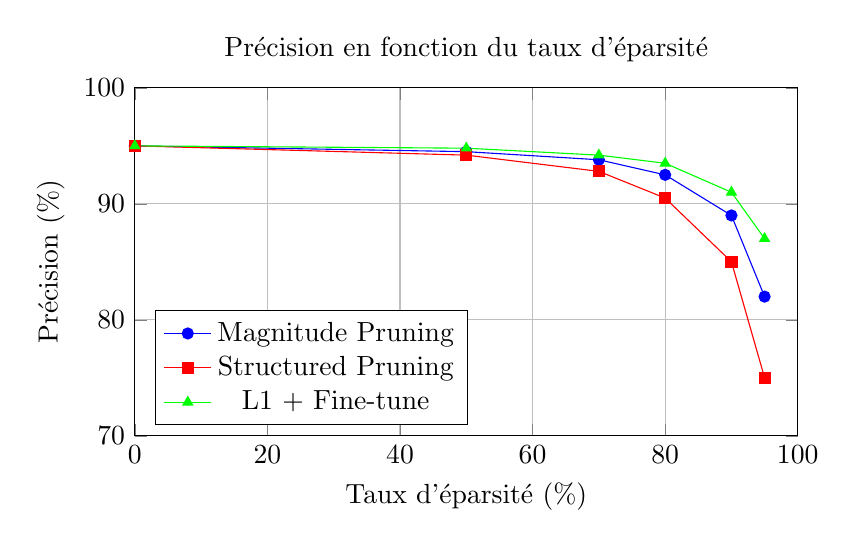
\begin{tikzpicture}
\begin{axis}[
    title={Précision en fonction du taux d'éparsité},
    xlabel={Taux d'éparsité (\%)},
    ylabel={Précision (\%)},
    xmin=0, xmax=100,
    ymin=70, ymax=100,
    grid=both,
    width=10cm,
    height=6cm,
    legend pos=south west
]

% Magnitude pruning
\addplot[blue, mark=*] coordinates {
    (0, 95.0)
    (50, 94.5)
    (70, 93.8)
    (80, 92.5)
    (90, 89.0)
    (95, 82.0)
};
\addlegendentry{Magnitude Pruning}

% Structured pruning
\addplot[red, mark=square*] coordinates {
    (0, 95.0)
    (50, 94.2)
    (70, 92.8)
    (80, 90.5)
    (90, 85.0)
    (95, 75.0)
};
\addlegendentry{Structured Pruning}

% L1 + Fine-tune
\addplot[green, mark=triangle*] coordinates {
    (0, 95.0)
    (50, 94.8)
    (70, 94.2)
    (80, 93.5)
    (90, 91.0)
    (95, 87.0)
};
\addlegendentry{L1 + Fine-tune}

\end{axis}
\end{tikzpicture}
\end{document}